%%%%%%%%%%%%%%%%%%%%%%%%%%%%%%%%%%%%%%%%%%%%%%%%%%%%%%
%%%%%%%%%%%%%%%%%%%%%%%%%%%%%%%%%%%%%%%%%%%%%%%%%%%%%%

\documentclass[xcolor=x11names,compress]{beamer}

\usepackage{biblatex}
\bibliography{main}

\usepackage{appendixnumberbeamer}
\usepackage{amsmath}
\usepackage{graphicx}
\usepackage{palatino}

\useoutertheme[subsection=false,shadow]{miniframes}
\useinnertheme{default}
\usefonttheme{serif}

\setbeamerfont{title like}{shape=\scshape}
\setbeamerfont{frametitle}{shape=\scshape}

\setbeamercolor*{lower separation line head}{bg=DeepSkyBlue4}
\setbeamercolor*{normal text}{fg=black,bg=white}
\setbeamercolor*{alerted text}{fg=red}
\setbeamercolor*{example text}{fg=black}
\setbeamercolor*{structure}{fg=black}
\setbeamercolor*{palette tertiary}{fg=black,bg=black!10}
\setbeamercolor*{palette quaternary}{fg=black,bg=black!10}

\setbeamertemplate{caption}[numbered]

%%%%%%%%%%%%%%%%%%%%%%%%%%%%%%%%%%%%%%%%%%%%%%%%%%%%%%
%%%%%%%%%%%%%%%%%%%%%%%%%%%%%%%%%%%%%%%%%%%%%%%%%%%%%%

\begin{document}

\beamertemplatenavigationsymbolsempty

\title{The Development of Purdue's Computerized Interactive Teaching Assistant}
\subtitle{The CITA on CHIP Project}
\author{
    Presenter: Cyrus Vandrevala\\
    \vspace{3mm}
    Committee: Lynn Bryan, Andrew Hirsch,\\
    Hisao Nakanishi, and Laura Pyrak-Nolte\\
    \vspace{3mm}
    {\it Purdue University}\\
}
\date{August 30, 2016}

%%%%%%%%%%%%%%%%%%%%%%%%%%%%%%%%%%%%%%%%%%%%%%%%%%%%%%
%%%%%%%%%%%%%%%%%%%%%%%%%%%%%%%%%%%%%%%%%%%%%%%%%%%%%%

\begin{frame}
    \titlepage
\end{frame}

%%%%%%%%%%%%%%%%%%%%%%%%%%%%%%%%%%%%%%%%%%%%%%%%%%%%%%
%%%%%%%%%%%%%%%%%%%%%%%%%%%%%%%%%%%%%%%%%%%%%%%%%%%%%%

\begin{frame}{Table of Contents}
    \tableofcontents
\end{frame}

%%%%%%%%%%%%%%%%%%%%%%%%%%%%%%%%%%%%%%%%%%%%%%%%%%%%%%
%%%%%%%%%%%%%%%%%%%%%%%%%%%%%%%%%%%%%%%%%%%%%%%%%%%%%%

\section{\scshape Background}

\subsection{Electricity and Optics}
\begin{frame}{frame 1}
    \begin{itemize}
    \item Item A
    \item Item B
    \begin{itemize}
    \item Subitem 1
    \item Subtem 2
    \end{itemize}
    \item Item C
    \end{itemize}
\end{frame}

%%%%%%%%%%%%%%%%%%%%%%%%%%%%%%%%%%%%%%%%%%%%%%%%%%%%%%
%%%%%%%%%%%%%%%%%%%%%%%%%%%%%%%%%%%%%%%%%%%%%%%%%%%%%%
\subsection{frame 2}
\begin{frame}{frame 2}

\end{frame}

%%%%%%%%%%%%%%%%%%%%%%%%%%%%%%%%%%%%%%%%%%%%%%%%%%%%%%
%%%%%%%%%%%%%%%%%%%%%%%%%%%%%%%%%%%%%%%%%%%%%%%%%%%%%%
\subsection{frame 3}
\begin{frame}{frame 3}

\end{frame}


%%%%%%%%%%%%%%%%%%%%%%%%%%%%%%%%%%%%%%%%%%%%%%%%%%%%%%
%%%%%%%%%%%%%%%%%%%%%%%%%%%%%%%%%%%%%%%%%%%%%%%%%%%%%%

\section{\scshape Methodology}
\subsection{frame 1}
\begin{frame}{frame 1}

\end{frame}


%%%%%%%%%%%%%%%%%%%%%%%%%%%%%%%%%%%%%%%%%%%%%%%%%%%%%%
%%%%%%%%%%%%%%%%%%%%%%%%%%%%%%%%%%%%%%%%%%%%%%%%%%%%%%
\subsection{frame 1}
\begin{frame}{frame 1}

\end{frame}

%%%%%%%%%%%%%%%%%%%%%%%%%%%%%%%%%%%%%%%%%%%%%%%%%%%%%%
%%%%%%%%%%%%%%%%%%%%%%%%%%%%%%%%%%%%%%%%%%%%%%%%%%%%%%

\section{\scshape Results}
\subsection{Frame 1}
\begin{frame}{Frame 1}

\end{frame}

%%%%%%%%%%%%%%%%%%%%%%%%%%%%%%%%%%%%%%%%%%%%%%%%%%%%%%
%%%%%%%%%%%%%%%%%%%%%%%%%%%%%%%%%%%%%%%%%%%%%%%%%%%%%%

\section{\scshape Conclusion}

\subsection{Summary}
\begin{frame}{Summary}
    \begin{itemize}
        \item We paired a number of tutorials with homework problems
        \item Thematic Analysis of Online Homework Systems
        \item Cupcake Physics
    \end{itemize}
\end{frame}

\subsection{Future Directions}
\begin{frame}{Future Directions}
    \begin{itemize}
        \item At Purdue
        \begin{itemize}
            \item Write Up Piazza Results
            \item Thematic Analysis of Online Homework Systems\ref{fig:overall_grade_vs_clicks_ap_students}
        \end{itemize}
        \vspace{3mm}
        \item For Me Personally
        \begin{itemize}
            \item Cupcake Physics
        \end{itemize}
    \end{itemize}
\end{frame}

%%%%%%%%%%%%%%%%%%%%%%%%%%%%%%%%%%%%%%%%%%%%%%%%%%%%%%
%%%%%%%%%%%%%%%%%%%%%%%%%%%%%%%%%%%%%%%%%%%%%%%%%%%%%%
\appendix
\section{\scshape Backup Slides}

\subsection{Small P-Value, Small $R^2$}
\begin{frame}{Frame 1}
 hi\footfullcite{test}
\end{frame}

\subsection{Overall Grade vs. Number of Clicks for AP Physics Students}
\begin{frame}{Overall Grade vs. Number of Clicks}
	\framesubtitle{AP Physics Students}
	\begin{figure}
		\centering
		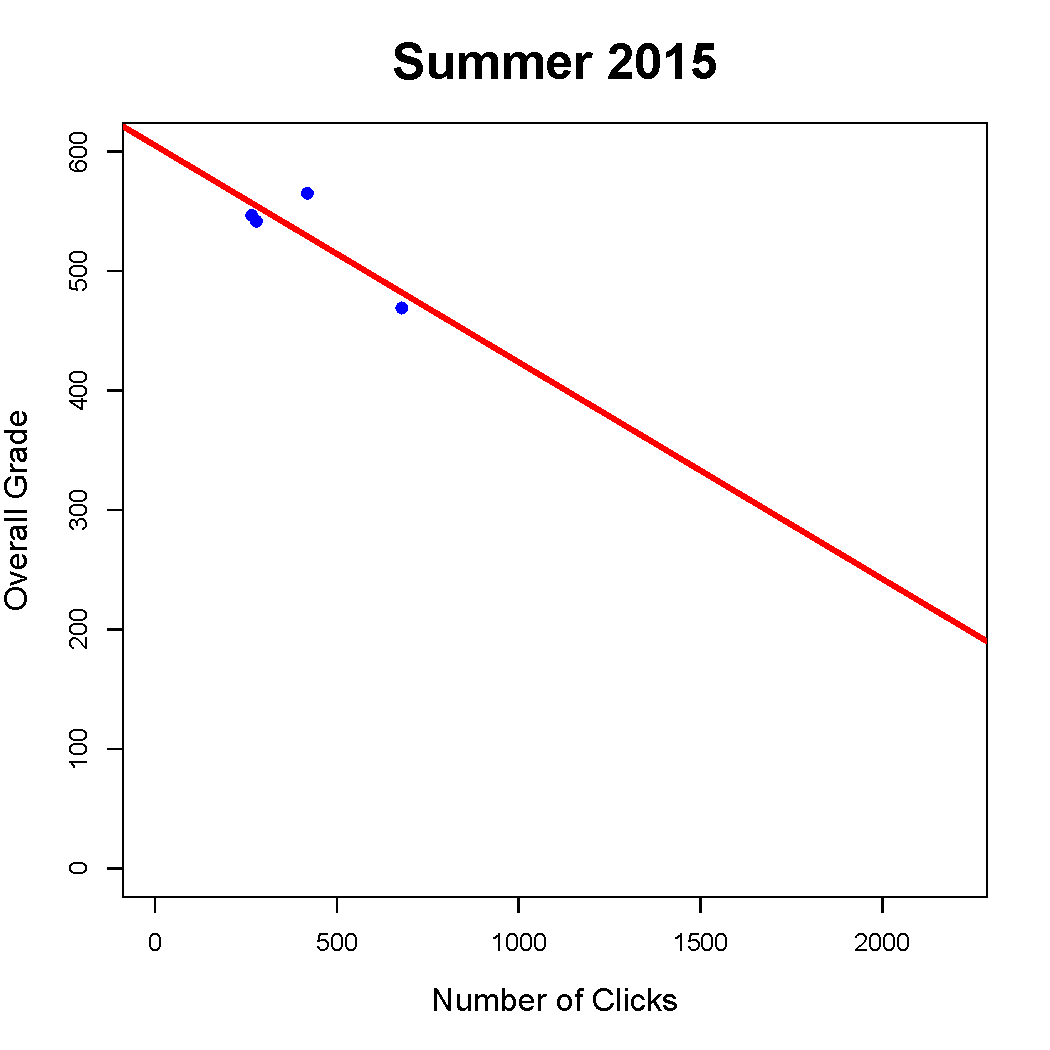
\includegraphics[width=0.33\textwidth]{img/overall_grade_vs_clicks_su15_ap_students.pdf}
		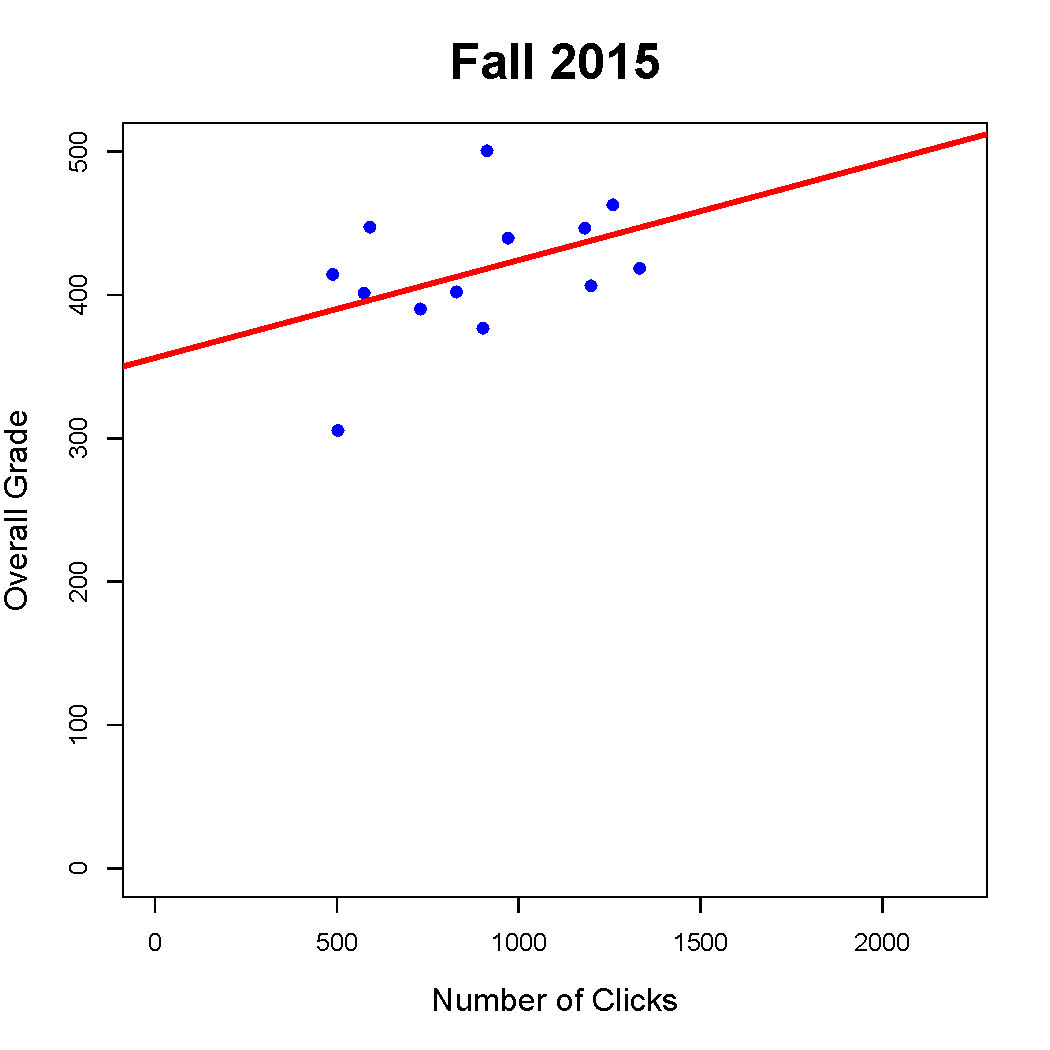
\includegraphics[width=0.33\textwidth]{img/overall_grade_vs_clicks_fa15_ap_students.pdf}
		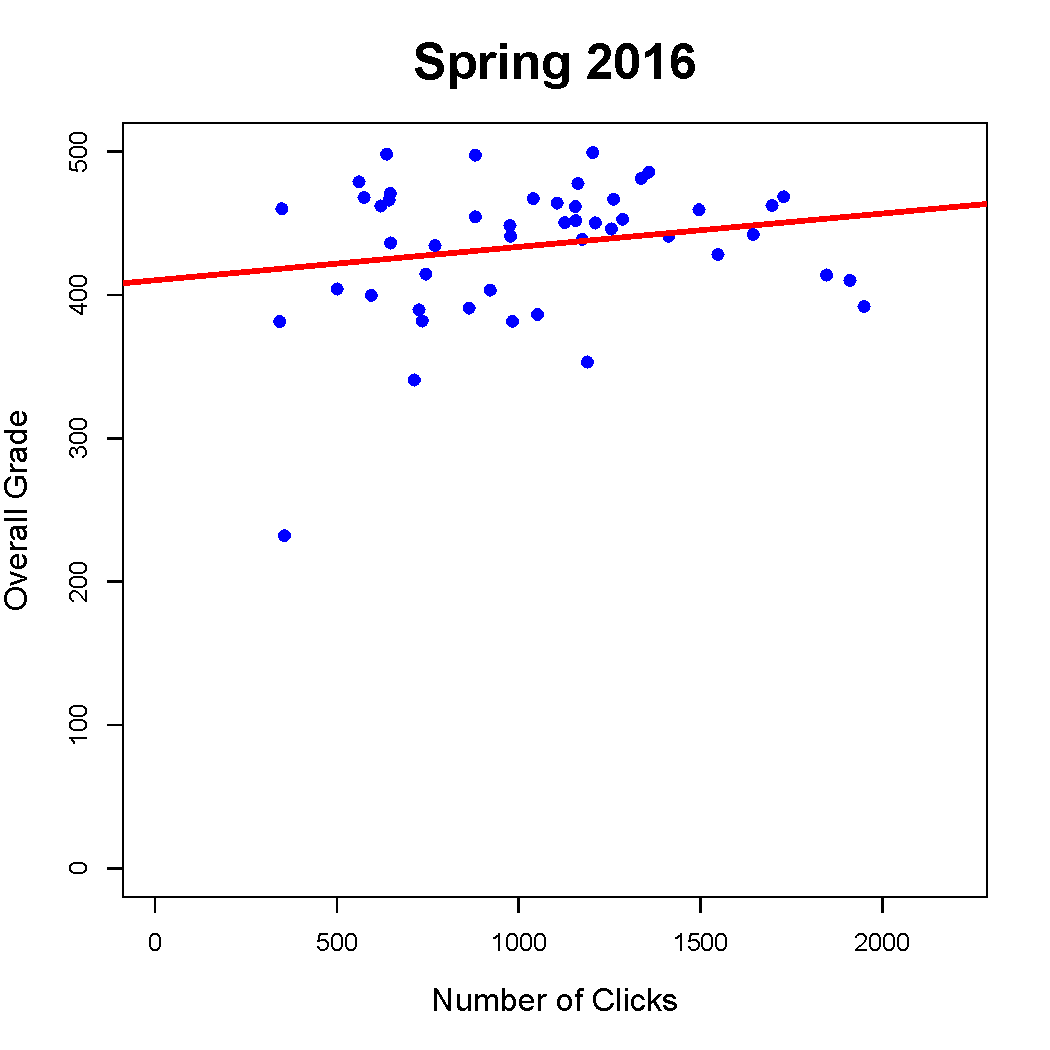
\includegraphics[width=0.33\textwidth]{img/overall_grade_vs_clicks_sp16_ap_students.pdf}
		\caption{In the summer and fall of 2015, a linear model did not fit the data due to the small sample sizes ($p = 0.177$ and $p = 0.146$, respectively). In the spring of 2016, a linear model did not fit the data due to the large range of Overall Grades ($p = 0.165$).}
		\label{fig:overall_grade_vs_clicks_ap_students}
	\end{figure}
\end{frame}

%%%%%%%%%%%%%%%%%%%%%%%%%%%%%%%%%%%%%%%%%%%%%%%%%%%%%%
%%%%%%%%%%%%%%%%%%%%%%%%%%%%%%%%%%%%%%%%%%%%%%%%%%%%%%

\end{document}
